\ifx\allfiles\undefined
\documentclass[12pt, a4paper,oneside, UTF8]{ctexbook}
\usepackage[dvipsnames]{xcolor}
\usepackage{amsmath}   % 数学公式
\usepackage{amsthm}    % 定理环境
\usepackage{amssymb}   % 更多公式符号
\usepackage{graphicx}  % 插图
%\usepackage{mathrsfs}  % 数学字体
%\usepackage{newtxtext,newtxmath}
%\usepackage{arev}
\usepackage{kmath,kerkis}
\usepackage{newtxtext}
\usepackage{bbm}
\usepackage{enumitem}  % 列表
\usepackage{geometry}  % 页面调整
%\usepackage{unicode-math}
\usepackage[colorlinks,linkcolor=black]{hyperref}

\usepackage{wrapfig}


\usepackage{ulem}	   % 用于更多的下划线格式,
					   % \uline{}下划线,\uuline{}双下划线,\uwave{}下划波浪线,\sout{}中间删除线,\xout{}斜删除线
					   % \dashuline{}下划虚线,\dotuline{}文字底部加点


\graphicspath{ {flg/},{../flg/}, {config/}, {../config/} }  % 配置图形文件检索目录
\linespread{1.5} % 行高

% 页码设置
\geometry{top=25.4mm,bottom=25.4mm,left=20mm,right=20mm,headheight=2.17cm,headsep=4mm,footskip=12mm}

% 设置列表环境的上下间距
\setenumerate[1]{itemsep=5pt,partopsep=0pt,parsep=\parskip,topsep=5pt}
\setitemize[1]{itemsep=5pt,partopsep=0pt,parsep=\parskip,topsep=5pt}
\setdescription{itemsep=5pt,partopsep=0pt,parsep=\parskip,topsep=5pt}

% 定理环境
% ########## 定理环境 start ####################################
\theoremstyle{definition}
\newtheorem{defn}{\indent 定义}[section]

\newtheorem{lemma}{\indent 引理}[section]    % 引理 定理 推论 准则 共用一个编号计数
\newtheorem{thm}[lemma]{\indent 定理}
\newtheorem{corollary}[lemma]{\indent 推论}
\newtheorem{criterion}[lemma]{\indent 准则}

\newtheorem{proposition}{\indent 命题}[section]
\newtheorem{example}{\indent \color{SeaGreen}{例}}[section] % 绿色文字的 例 ,不需要就去除\color{SeaGreen}{}
\newtheorem*{rmk}{\indent \color{red}{注}}

% 两种方式定义中文的 证明 和 解 的环境:
% 缺点:\qedhere 命令将会失效【技术有限,暂时无法解决】
\renewenvironment{proof}{\par\textbf{证明.}\;}{\qed\par}
\newenvironment{solution}{\par{\textbf{解.}}\;}{\qed\par}

% 缺点:\bf 是过时命令,可以用 textb f等替代,但编译会有关于字体的警告,不过不影响使用【技术有限,暂时无法解决】
%\renewcommand{\proofname}{\indent\bf 证明}
%\newenvironment{solution}{\begin{proof}[\indent\bf 解]}{\end{proof}}
% ######### 定理环境 end  #####################################

% ↓↓↓↓↓↓↓↓↓↓↓↓↓↓↓↓↓ 以下是自定义的命令  ↓↓↓↓↓↓↓↓↓↓↓↓↓↓↓↓

% 用于调整表格的高度  使用 \hline\xrowht{25pt}
\newcommand{\xrowht}[2][0]{\addstackgap[.5\dimexpr#2\relax]{\vphantom{#1}}}

% 表格环境内长内容换行
\newcommand{\tabincell}[2]{\begin{tabular}{@{}#1@{}}#2\end{tabular}}

% 使用\linespread{1.5} 之后 cases 环境的行高也会改变,重新定义一个 ca 环境可以自动控制 cases 环境行高
\newenvironment{ca}[1][1]{\linespread{#1} \selectfont \begin{cases}}{\end{cases}}
% 和上面一样
\newenvironment{vx}[1][1]{\linespread{#1} \selectfont \begin{vmatrix}}{\end{vmatrix}}

\def\d{\textup{d}} % 直立体 d 用于微分符号 dx
\def\R{\mathbb{R}} % 实数域
\def\N{\mathbb{N}} % 自然数域
\def\C{\mathbb{C}} % 复数域
\def\Z{\mathbb{Z}} % 整数环
\def\Q{\mathbb{Q}} % 有理数域
\newcommand{\bs}[1]{\boldsymbol{#1}}    % 加粗,常用于向量
\newcommand{\ora}[1]{\overrightarrow{#1}} % 向量

% 数学 平行 符号
\newcommand{\pll}{\kern 0.56em/\kern -0.8em /\kern 0.56em}

% 用于空行\myspace{1} 表示空一行 填 2 表示空两行  
\newcommand{\myspace}[1]{\par\vspace{#1\baselineskip}}

%s.t. 用\st就能打出s.t.
\DeclareMathOperator{\st}{s.t.}

%罗马数字 \rmnum{}是小写罗马数字, \Rmnum{}是大写罗马数字
\makeatletter
\newcommand{\rmnum}[1]{\romannumeral #1}
\newcommand{\Rmnum}[1]{\expandafter@slowromancap\romannumeral #1@}
\makeatother
\begin{document}
	% \title{{\Huge{\textbf{$Real \,\, Analysis$}}}\\
		\Large{\textbf{$Measure \,\, Theory , \,\, Integration , \,\, \& \,\, Hilbert \,\, Spaces$}}\footnote{参考书籍:\\
			\hspace*{4em} \textbf{《$Real \,\, Analysis -- Measure \,\, Theroy, \,\, Integration, \,\, \& \,\, Hilbert \,\, Spaces$》--- $Elias \,\, M. \,\, Stein$} \\
			\hspace*{4em} \textbf{《$Real \,\, Analysis -- Modern \,\, Techniques \,\, and \,\, Their \,\, Applications$》--- $Gerald \,\, B. \,\, Folland$}}}
\author{$-TW-$}
\date{\today}
\maketitle                   % 在单独的标题页上生成一个标题

\thispagestyle{empty}        % 前言页面不使用页码
\begin{center}
	\Huge\textbf{序}
\end{center}


\vspace*{3em}
\begin{center}
	\large{\textbf{天道几何,万品流形先自守;}}\\
	
	\large{\textbf{变分无限,孤心测度有同伦。}}
\end{center}

\vspace*{3em}
\begin{flushright}
	\begin{tabular}{c}
		\today \\ \small{\textbf{长夜伴浪破晓梦,梦晓破浪伴夜长}}
	\end{tabular}
\end{flushright}


\newpage                      % 新的一页
\pagestyle{plain}             % 设置页眉和页脚的排版方式(plain:页眉是空的,页脚只包含一个居中的页码)
\setcounter{page}{1}          % 重新定义页码从第一页开始
\pagenumbering{Roman}         % 使用大写的罗马数字作为页码
\tableofcontents              % 生成目录

\newpage                      % 以下是正文
\pagestyle{plain}
\setcounter{page}{1}          % 使用阿拉伯数字作为页码
\pagenumbering{arabic}
\setcounter{chapter}{0}    % 设置 -1 可作为第零章绪论从第零章开始 
	\else
	\fi
	%  ############################ 正文部分
\chapter{$Differentiation \,\, and \,\, Integration$}
\paragraph{\textbf{Motivation}}
	在\textbf{Riemann积分}的框架下,我们知道\textbf{积分}和\textbf{微分}可以视作一对互逆的运算. 而在这一章,我们将在全新的\textbf{Lebesgue测度}的框架下重新审视\textbf{积分}和\textbf{微分}之间的关系.
	
	\vspace{1em}
	下面先来描述一下想要解决的问题.
	\begin{itemize}
		\item Let $f \in \mathcal{L}^{1}(\R^d)$. 对于\textbf{变上限积分}$F(x) = \int_{a}^{x}{f(y) dy}$,我们知道根据\textbf{Riemann积分下的微积分基本定理},对$F$求导就会回到被积函数$f$ 本身. 那么我们就会好奇:
		
		\vspace{1em}
		
		\begin{itemize}
			\item 在\textbf{Lebesgue积分}的框架下,这个结论是否还成立?
			
			\item 如果成立的话,又对哪些$x$成立呢?
		\end{itemize}
	
		\vspace{1em}
		
		此时回顾求导的定义,即对于差商 (此处改写为更具一般性的符号$I = (x , x + h)$)
		\begin{align}
			\frac{F(x + h) - F(x)}{h} 
			= \frac{1}{h} \int_{x}^{x + h}{f(y) dy} 
			= \frac{1}{\left| I \right|} \int_{I}{f(y) dy}
		\end{align}
		对差商中的增量$h \to 0$,即得到\textbf{导数}的定义. 那么我们的问题就转化为了
		\begin{align}
			\lim_{\substack{\left| I \right| \to 0 \\ I \ni x}}{\frac{1}{\left| I \right|} \int_{I}{f(y) dy}}
			= f(x) 
			\,\,\,\, \text{holds for which $x$?}
		\end{align}
	
		\vspace{1em}
		
		更一般地,将上述问题从一维实直线$\R$ 推广至$\R^d$ 空间上,将区间$I$ 用开球$B$ 替换,得
		\begin{align}
			\lim_{\substack{m(B) \to 0 \\ B \ni x}}{\frac{1}{m(B)} \int_{B}{f(y) dy}}
			= f(x)
			\,\,\,\, \text{holds for which $x$?}
		\end{align}
	
		\vspace{1em}
		
		\begin{rmk}
			\begin{itemize}
				\item 此处看似是随着开球$B$的测度减小,$x \in B$ 在跟着$B$ ``跑",但实际上则相反:
				\begin{center}
					对于每个固定的$x$,让包含着$x$ 的球$B \ni x$ 不断减小其测度,最后取极限 
				\end{center}	
				而这也就是此处极限条件写为``$B \ni x$" 而非``$x \in B$" 的原因,逻辑更清晰.
				
				\vspace{1em}
				
				\item 事实上该结论对于\textbf{几乎处处的$x$} 都成立 (若$f$ \textbf{Lebesgue可积}),这就是后面要讲的\textbf{Lebesgue微分定理}.
			\end{itemize}
		\end{rmk}
	\end{itemize}
	
\newpage
\section{$Hardy-Littlewood$ 极大函数}
\paragraph{定义}
	下面我们给出\textbf{Hardy-Littlewood 极大函数}的定义.
	\begin{defn}\label{def 4.1.1}
		If $f \in \mathcal{L}^{1}(\R^d)$, we define its \underline{\textcolor{blue}{\textbf{maximal function}}} $Mf$ by
		\begin{align}
			Mf(x) = \sup_{B \ni x}{\frac{1}{m(B)} \int_{B}{\left| f(y) \right| dy}}
		\end{align}
	
		\vspace{1em}
		\begin{rmk}
			我们目前并不知道球面测度的具体数值与计算方法,但事实上我们也并不需要知道其具体数值,具体表现在: \\
			设$\R^d$ 中单位球$B(0 , 1)$ 的测度为$m(B(0 , 1)) = v_d$. $\forall B(x , r) \subset \R^d$,根据\textbf{Lebesgue测度的平移不变性和伸缩变换公式 (Prop \ref{prop 3.7.1})}
			\begin{center}
				$B(0 , r) = r B(0 , 1) \,\, \Rightarrow \,\, m(B(x , r)) = m(B(0 , r)) = r^d m(B(0 , 1)) = r^d v_d$
			\end{center}
		\end{rmk}
	\end{defn}

\vspace{2em}
\paragraph{性质}
	下面来说明\textbf{Hardy-Littlewood 极大函数}的三条\textbf{性质}.
	\begin{proposition}\label{prop 4.1.1}
		Suppose $f \in \mathcal{L}^{1}(\R^d)$. Then:
		\begin{enumerate}
			\item[(\rmnum{1})]$Mf$ is measurable.
			
			\item[(\rmnum{2})]$Mf(x) < \infty$ for a.e. $x$.
			
			\item[(\rmnum{3})]\textbf{weak-type inequality}. \\
			$Mf$ satisfies
			\begin{align}
				m\left( \left\{ x \in \R^d \mid Mf(x) > \alpha \right\} \right) 
				\leq \frac{A}{\alpha} \,\, \Vert f \Vert_{\mathcal{L}^1} , \,\, \forall \alpha > 0
			\end{align}
			where $A = 3^d$.
		\end{enumerate}
	
		\vspace{4em}
		\begin{proof}
			\begin{enumerate}
				\item [(\rmnum{1})]Let $E_\alpha = \{ x \in \R^d \mid Mf(x) > \alpha \}$. 下面证明$E_\alpha$ open. \\
				$\forall x \in E_\alpha$, by the \textbf{definition of $Mf$ (Def \ref{def 4.1.1})}, $\exists B_x \ni x$, $\st$
				\begin{align}
					\frac{1}{m(B_x)} \int_{B_x}{\left| f \right|} > \alpha
				\end{align}
				Then $\forall y \in B_x$, $B_x$ is also an open ball containing $y$, so we have $y \in E_\alpha$. i.e. $B_x \subset E_\alpha$. \\
				Therefore, $E_\alpha$ is open, specifically measurable for all $\alpha$. Then $Mf$ is measurable.
				
				\newpage
				
				\item[(\rmnum{2})]下面说明(\rmnum{3}) $\Rightarrow$ (\rmnum{2}): \\
				Let $E_\alpha = \{ x \in \R^d \mid Mf(x) > \alpha \}$. Then $E_n \searrow E = \{ x \in \R^d \mid Mf(x) = \infty \}$. \\
				Since $f \in \mathcal{L}^{1}(\R^d)$, $\Vert f \Vert_{\mathcal{L}^1}$ is finite. Then by \textbf{(\rmnum{3})}, $m(E_1) < \infty$. \\
				Then by \textbf{Thm \ref{thm 1.3.3}},
				\begin{align}
					m(E) = \lim_{n \to \infty}{m(E_n)} \leq \lim_{n \to \infty}{\frac{A}{n} \,\, \Vert f \Vert_{\mathcal{L}^1}} = 0
				\end{align}
				Therefore $m(E) = 0$. i.e. $Mf(x) < \infty$ for a.e. $x$.
				
				\vspace{6em}
				
				\item[(\rmnum{3})]在证明(\rmnum{3})之前,先来介绍\textbf{Vitali覆盖引理}.
				
				\vspace{2em}
				
				\begin{lemma}\label{lemma 4.1.1}
					\textbf{Vitali Covering Lemma (Elementary Version)}. \\
					Suppose $\mathcal{B} = \{ B_1 , B_2 , \cdots , B_N \}$, $B_i \subset \R^d$ are open balls, then there is a disjoint subcollection $B_{i_1} , \cdots , B_{i_k}$ that satisfies
					\begin{align}
						m\left( \bigcup_{l = 1}^{N}{B_l} \right) 
						\leq 3^d \sum_{j = 1}^{k}{m(B_{i_j})}
					\end{align}
					
					\vspace{1em}
					\begin{rmk}
						这是\textbf{Vitali覆盖引理}的\textbf{初等版本 (有限版本)},更一般的版本是对\textbf{一列}球结论成立.
					\end{rmk}
				
					\vspace{1em}
					\begin{proof}
						详见视频\href{https://www.bilibili.com/video/BV1FT411C7wM?p=31}{(非球心)Hardy-Littlewood极大函数} 23:10 (类似\textbf{贪心算法}的迭代步骤)
					\end{proof}
					
					\begin{figure}[thbp!]
						\centering
						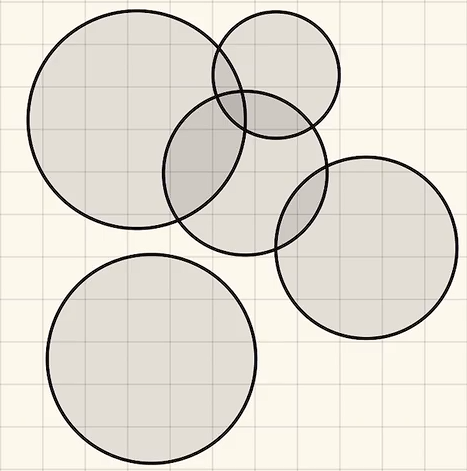
\includegraphics[width=0.25\linewidth]{figure/4.1.1-1}
						\caption{Lemma 4.1.1}
						\label{pic : 4.1.1-1} % 添加图像引用标签
					\end{figure}
				\end{lemma}
			
				\newpage
				
				下面继续来证明(\rmnum{3}): \\
				Fix $\alpha > 0$, $\forall x \in B_\alpha$, $\exists$ open ball $B_x$, $\st$
				\begin{align}
					\frac{1}{m(B_x)} \int_{B_x}{\left| f \right|} > \alpha
				\end{align}
				So we have $E_\alpha \subset \underset{x \in E_\alpha}{\bigcup}{B_x}$. \\
				Since $E_\alpha$ is measurable (by \textbf{(\rmnum{1})}), then by \textbf{Thm \ref{thm 1.3.4} (Lebesgue测度的内正则性)}, \\
				$\forall \epsilon > 0$, $\exists$ compact $K_\epsilon \subset E_\alpha$, $\st$
				\begin{center}
					$m(E_\alpha \backslash K_\epsilon) \leq \epsilon$
				\end{center}
				i.e.
				\begin{center}
					$m(E_\alpha) - m(K_\epsilon) \leq \epsilon$
				\end{center}
				Since $K_\epsilon$ is compact, $K_\epsilon \subset \underset{x \in K_\epsilon}{\bigcup}{B_x}$, there exists a subcollection $B_{x_1} , \cdots , B_{x_N}$, $\st$
				\begin{center}
					$K_\epsilon \subset \overset{N}{\underset{l = 1}{\bigcup}}{B_{x_l}}$
				\end{center}
				Then by \textbf{Vitali Covering Lemma (Lemma \ref{lemma 4.1.1})}, there exists a subcollection $B_{x_{i_1}} , \cdots , B_{x_{i_k}}$, $\st$
				\begin{center}
					$m\left( \overset{N}{\underset{l = 1}{\bigcup}}{B_{x_l}} \right) 
					\leq 3^d \overset{k}{\underset{j = 1}{\sum}}{m(B_{x_{i_j}})}$
				\end{center}
				Therefore
				\begin{align}
					m(K_\epsilon) 
					\leq m\left( \bigcup_{l = 1}^{N}{B_{x_l}} \right)
					&\leq 3^d \sum_{j = 1}^{k}{m(B_{x_{i_j}})} \\
					&= \frac{3^d}{\alpha} \sum_{j = 1}^{k}{\alpha \cdot m(B_{x_{i_j}})} \\
					&\leq \frac{3^d}{\alpha} \int_{\bigcup_{j = 1}^{k}{B_{x_{i_j}}}}{\left| f \right|} \\
					&\leq \frac{3^d}{\alpha} \int_{\R^d}{\left| f \right|} \\
					&= \frac{3^d}{\alpha} \,\, \Vert f \Vert_{\mathcal{L}^1}
				\end{align}
				Then
				\begin{align}
					m(E_\alpha) 
					\leq m(K_\epsilon) + \epsilon 
					\leq \frac{A}{\alpha} \,\, \Vert f \Vert_{\mathcal{L}^1} + \epsilon
				\end{align}
				where $A = 3^d$, $\epsilon > 0$. \\
				Since $\epsilon$ is arbitrary, let $\epsilon \to 0$, we have
				\begin{align}
					m(E_\alpha) \leq \frac{A}{\alpha} \,\, \Vert f \Vert_{\mathcal{L}^1} , \,\, A = 3^d , \,\, \forall \alpha > 0
				\end{align}
			\end{enumerate}
		\end{proof}
	\end{proposition}

\newpage
\section{$Lebesgue$ 微分定理}
	\begin{center}
		在这一节我们将利用\textbf{Hardy-Littlewood极大函数}来证明\textbf{Lebesgue微分定理}.
	\end{center}
	
\subsection{$Chebyshev's \,\, Inequality$}
	在此之前,我们先来证明一个非常有用的不等式,即\textbf{切比雪夫不等式}.
	\begin{thm}\label{thm 4.2.1}
		\textbf{Chebyshev's Inequality}. \\
		If $g \in \mathcal{L}^{1}(\R^d)$, then
		\begin{align}
			m\left( \left\{ x \in \R^d \mid \left| g(x) \right| > \alpha \right\} \right)
			\leq \frac{1}{\alpha} \,\, \Vert g \Vert_{\mathcal{L}^1} , \,\, \forall \alpha > 0
		\end{align}
		
		\vspace{4em}
		\begin{proof}
			Let $E_\alpha = \{ x \in \R^d \mid \left| g(x) \right| > \alpha \}$. Then
			\begin{align}
				\Vert g \Vert_{\mathcal{L}^1}
				= \int_{\R^d}{\left| g \right|}
				\geq \int_{E_\alpha}{\left| g \right|}
				\geq \int_{E_\alpha}{\alpha}
				= \alpha \cdot m(E_\alpha)
			\end{align}
		\end{proof}
	\end{thm}

\newpage
\subsection{$The \,\, Lebesgue \,\, Differentiation \,\, Theorem$}
	下面我们就来给出\textbf{Lebesgue微分定理}.
	\begin{thm}\label{thm 4.2.2}
		If $f \in \mathcal{L}^{1}(\R^d)$, then
		\begin{align}
			\lim_{\substack{m(B) \to 0 \\ B \ni x}}{\frac{1}{m(B)} \int_{B}{f(y) dy}} = f(x) \,\,\,\, for \,\, a.e. \,\, x
		\end{align}
		
		\vspace{2em}
		\begin{rmk}
			\begin{itemize}
				\item \textbf{Lebesgue微分定理}说明了对于\textbf{几乎处处的$x$},当包含$x$ 的球体$B$ 的测度趋于0时,$f$ 在球体$B$ 上积分的平均值就会收敛到$f(x)$.
				
				\vspace{2em}
				
				\item 定理左侧实际上是关于集合$B$ 的函数的一个极限过程,用$\epsilon-\delta$语言叙述如下:\\
				$\forall \epsilon > 0$, $\exists \delta> 0$, $\st$ for all $B \ni x$ and $m(B) < \delta$, we have
				\begin{align}
					\left| \frac{1}{m(B)} \int_{B}{f(y) dy} - f(x) \right| \leq \epsilon
				\end{align}
			
				\vspace{2em}
				
				\item 要证明该定理,首先需要说明等式左侧\textbf{极限的存在性},但这并不好说明. 为了跳过说明其存在性的问题,我们需要引入类似\textbf{``上极限"}的函数,即: \\
				If suffices to show
				\begin{align}
					\lim_{\delta \to 0}{\sup_{\substack{m(B) < \delta \\ B \ni x}}{\left| \frac{1}{m(B)} \int_{B}{f(y) dy} - f(x) \right|}} = 0 \,\,\,\, for \,\, a.e. \,\, x
				\end{align}
				由于极限内的函数随着$\delta$ 递减而单调递减,又存在下界$0$,因此在$\delta = 0$ 处必存在右极限. 这样就跳过了原极限是否存在的问题.
				
				\vspace{2em}
				
				\item 事实上此处极限\textbf{``怪异"}的本质原因在于开球$B$ 的选取的任意性,若将其定义为以$x$ 为球心, $r$ 为半径的球,则可直接令$r \to 0$ 变为正常的函数极限,即
				\begin{align}
					\lim_{r \to 0}{\frac{1}{m(B(x , r))} \int_{B(x , r)}{f(y) dy}} = f(x)
				\end{align}
				在下一节我们会从\textbf{Hardy-Littlewood极大函数}开始,以此方法重新说明\textbf{Lebesgue微分定理}.
			\end{itemize}
		\end{rmk}
	
		\newpage
		\begin{proof}
			Let 
			\begin{align}
				E_\alpha 
				= \left\{ x \in \R^d \mid \lim_{\delta \to 0}{\sup_{\substack{m(B) < \delta \\ B \ni x}}{\left| \frac{1}{m(B)} \int_{B}{f(y) dy} - f(x) \right| > 2 \alpha}} \right\}
			\end{align}
			Then we \textbf{WTS (want to show)}:
			\begin{center}
				$m(E_\alpha) = 0$, $\forall \alpha \geq 0$
			\end{center}
			
			\vspace{1em}
			
			Fix $\alpha \geq 0$. By \textbf{Thm \ref{thm 3.2.3}}, $C_{c}(\R^d)$ is dense in $\mathcal{L}^{1}(\R^d)$ (有紧支集的连续函数), then \\
			$\forall \epsilon > 0$, $\exists g \in C_{c}(\R^d)$, $\st$
			\begin{center}
				$\Vert f - g \Vert_{\mathcal{L}^1} < \epsilon$
			\end{center}
			Since $g$ is uniformly continuous, then $\exists \delta > 0$, $\st$
			\begin{align}
				\left| \frac{1}{m(B)} \int_{B}{g(y) dy} - g(x) \right| 
				\leq \frac{1}{m(B)} \int_{B}{\left| g(y) - g(x) \right| dy}
				< \frac{1}{m(B)} \int_{B}{\epsilon dy} 
				= \epsilon
			\end{align}
			for all $B \ni x$ and $m(B) < \delta$. 
			
			\vspace{2em}
			
			下面对$m(E_\alpha)$ 进行估计. $\forall x \in E_\alpha$,
			\begin{align}
				\left| \frac{1}{m(B)} \int_{B}{f(y) dy} - f(x) \right|
				\leq \left| \frac{1}{m(B)} \int_{B}{(f(y) - g(y)) dy} \right|
				+ \left| \frac{1}{m(B)} \int_{B}{g(y) dy} - g(x) \right|
				+ \left| g(x) - f(x) \right|
			\end{align}
			对上述不等式中的开球$B \ni x$ 取上确界$\sup$,得
			\begin{align}
				\sup_{B \ni x}{\left| \frac{1}{m(B)} \int_{B}{f(y) dy} - f(x) \right|}
				\leq \sup_{B \ni x}{\left| \frac{1}{m(B)} \int_{B}{(f(y) - g(y)) dy} \right|}
				+ \sup_{B \ni x}{\left| \frac{1}{m(B)} \int_{B}{g(y) dy} - g(x) \right|}
				+ \left| g(x) - f(x) \right|
			\end{align}
			再令$m(B) \to 0$,由于根据\textbf{式 (4.24)},
			\begin{align}
				\lim_{\delta \to 0}{\sup_{\substack{m(B) < \delta \\ B \ni x}}{\left| \frac{1}{m(B)} \int_{B}{g(y) dy} - g(x) \right|}} = 0
			\end{align}
			因此
			\begin{align}
				\lim_{\delta \to 0}{\sup_{\substack{m(B) < \delta \\ B \ni x}}{\left| \frac{1}{m(B)} \int_{B}{f(y) dy} - f(x) \right|}}
				\leq \textcolor{red}{\lim_{\delta \to 0}{\sup_{\substack{m(B) < \delta \\ B \ni x}}{\left| \frac{1}{m(B)} \int_{B}{(f(y) - g(y)) dy} \right|}}}
				+ 0
				+ \left| g(x) - f(x) \right|
			\end{align}
			下面对\textcolor{red}{\textbf{红色部分}}进行估计. 根据对$\delta$ 的单调性可知,
			\begin{align}
				\textcolor{red}{\lim_{\delta \to 0}{\sup_{\substack{m(B) < \delta \\ B \ni x}}{\left| \frac{1}{m(B)} \int_{B}{(f(y) - g(y)) dy} \right|}}}
				\leq \sup_{B \ni x}{\frac{1}{m(B)} \int_{B}{\left| f(y) - g(y) \right| dy}}
				= M(f - g)(x)
			\end{align}
			又因为对于$\forall x \in E_\alpha$,
			\begin{align}
				\lim_{\delta \to 0}{\sup_{\substack{m(B) < \delta \\ B \ni x}}{\left| \frac{1}{m(B)} \int_{B}{f(y) dy} - f(x) \right|}}
				> 2 \alpha
			\end{align}
			所以
			\begin{align}
				&M(f - g)(x) + \left| g(x) - f(x) \right| > 2\alpha \\
				&\Rightarrow M(f - g)(x) > \alpha \,\, or \,\, \left| g(x) - f(x) \right| > \alpha \\
				&\Rightarrow E_\alpha 
				\subset \textcolor{purple}{\left\{ x \in \R^d \mid M(f - g)(x) > \alpha \right\}}
				\cup \textcolor{orange}{\left\{ x \in \R^d \mid \left| g - f \right| > \alpha \right\}}
			\end{align}
			下面分别来估计the \textcolor{purple}{\textbf{purple}} one 和 the \textcolor{orange}{\textbf{orange}} one 的测度.
			
			\vspace{2em}
			
			\begin{itemize}
				\item 由于$\left| f - g \right| \in \mathcal{L}^{1}{\R^d}$,因此根据\textbf{Chebyshev's Inequality (Thm \ref{thm 4.2.1})},
				\begin{align}
					m\left( \textcolor{orange}{\left\{ x \in \R^d \mid \left| g - f \right| > \alpha \right\}} \right)
					\leq \frac{1}{\alpha} \,\, \Vert f - g \Vert_{\mathcal{L}^1}
				\end{align}
				
				\vspace{1em}
				
				\item 根据\textbf{Hardy-Littlewood极大函数的weak-type inequality (Prop \ref{prop 4.1.1} (\rmnum{3}))},
				\begin{align}
					m\left( \textcolor{purple}{\left\{ x \in \R^d \mid M(f - g)(x) > \alpha \right\}} \right)
					\leq \frac{A}{\alpha} \,\, \Vert f - g \Vert_{\mathcal{L}^1}
				\end{align}
			\end{itemize}
		
			\vspace{2em}
			
			从而根据$\Vert f - g \Vert_{\mathcal{L}^1} < \epsilon$,
			\begin{align}
				m(E_\alpha)
				&\leq m\left( \textcolor{purple}{\left\{ x \in \R^d \mid M(f - g)(x) > \alpha \right\}} \right)
				+ m\left( \textcolor{orange}{\left\{ x \in \R^d \mid \left| g - f \right| > \alpha \right\}} \right) \\
				&\leq \frac{A + 1}{\alpha} \,\, \Vert f - g \Vert_{\mathcal{L}^1} \\
				&< \frac{A + 1}{\alpha} \epsilon , \,\, \forall \alpha \geq 0
			\end{align}
			Since $\epsilon > 0$ is arbitrary, let $\epsilon \to 0$, we get
			\begin{align}
				m(E_\alpha) = 0 , \,\, \forall \alpha \geq 0
			\end{align}
		\end{proof}
	\end{thm}


	%  ############################
	\ifx\allfiles\undefined
\end{document}
\fi